\section{Subdivision Surfaces}

\greenbf{Corner Cutting:} Insert two new vertices at $\frac{1}{4}$ and $\frac{3}{4}$ of each edge. Remove old and connect new vertices.
\includegraphics*[width = \columnwidth]{alex/cornerCutting.png}

\greenbf{Subdivision surfaces:} Generalisation of spline curves/surfaces, arbitrary control meshes, successive refinement, converges to smooth limit surface, connection between splines and meshes. In a sense similar to deCasteljau (corner cutting). No regular structure like curves (arbitrary number of edge neighbours, different subdivision rules for each valence). \\
\textbf{Classification:} Primal: faces are split into sub-faces. Dual: Vertices are split into multiple vertices. Approximating: Control points not interpolated. Interpolating: Control points interpolated.\\
\includegraphics*[width = \columnwidth]{alex/subdivisionClassification.png}\\
\greenbf{Doo-Sabin:} 
\raisebox{-1ex}{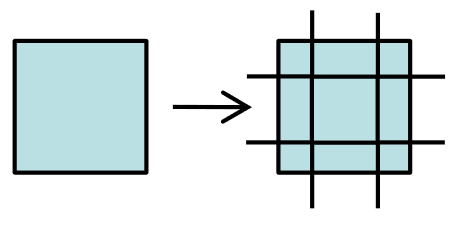
\includegraphics[height= 3ex]{assets/arjun/doo-sabin-icon.png}}
generalisation of bi-quadratic B-Splines, for polygonal meshes, generates $G^1$ continuous surfaces.\\
\greenbf{Catmull-Clark:} \raisebox{-1ex}{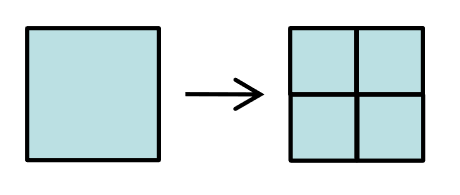
\includegraphics[height= 3ex]{assets/arjun/catmull-clark-icon.png}} generalisation of bi-cubic B-Spline, polygonal meshes, $G^2$\\
\greenbf{Loop Subdivision:} 
\raisebox{-1ex}{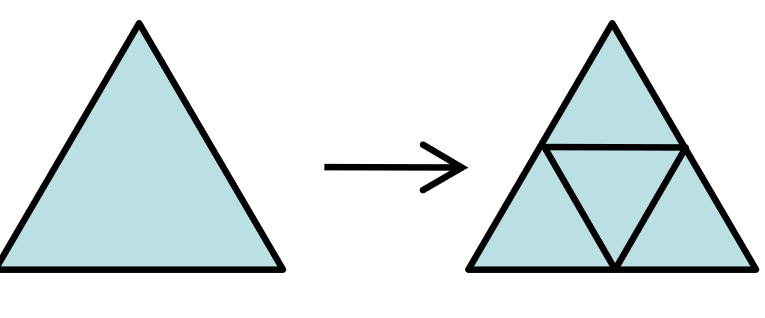
\includegraphics[height= 3ex]{assets/arjun/loop-subdivision-icon.png}} generalisation of box splines, triangle meshes, $G^2$\\
\greenbf{Butterfly:} triangle meshes, $G^1$ continuous\\
Top row: Start, Doo-Sabin, Catmull-Clark. \\
Bottom-row: Start, Loop Subdivision, Butterfly \\
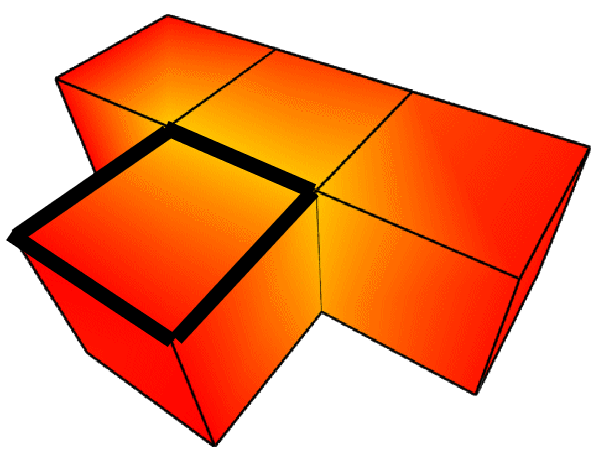
\includegraphics[width=0.3\columnwidth]{assets/arjun/start-square.png}
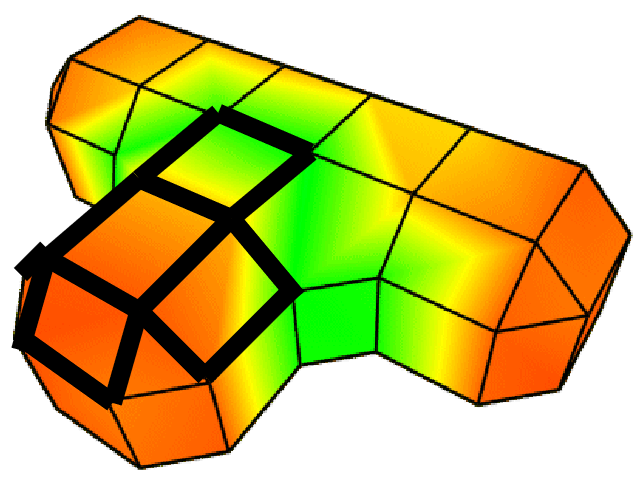
\includegraphics[width=0.3\columnwidth]{assets/arjun/doo-sabin.png}
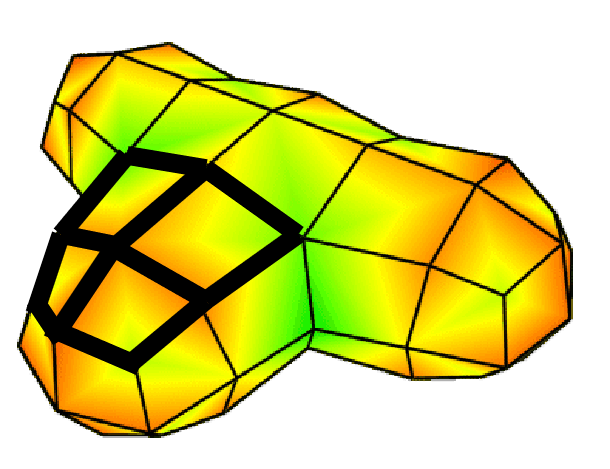
\includegraphics[width=0.3\columnwidth]{assets/arjun/catmull-clark.png}
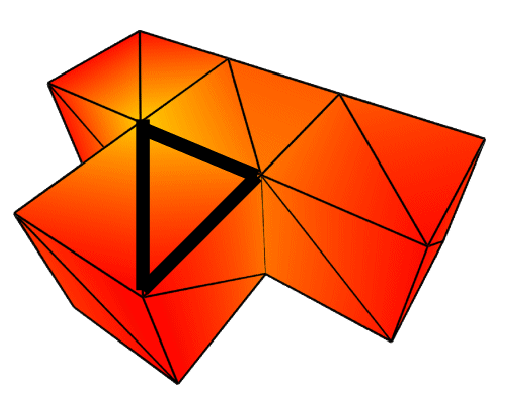
\includegraphics[width=0.3\columnwidth]{assets/arjun/start-triangle.png}
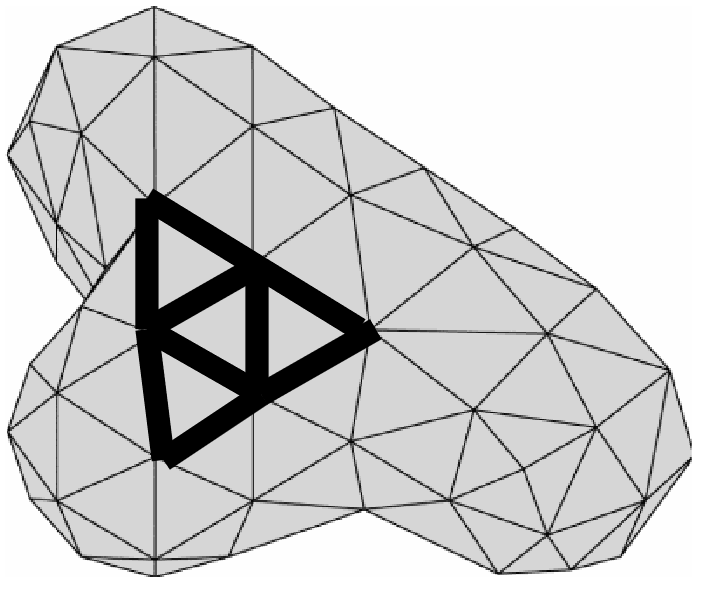
\includegraphics[width=0.3\columnwidth]{assets/arjun/loop-subdivision.png}
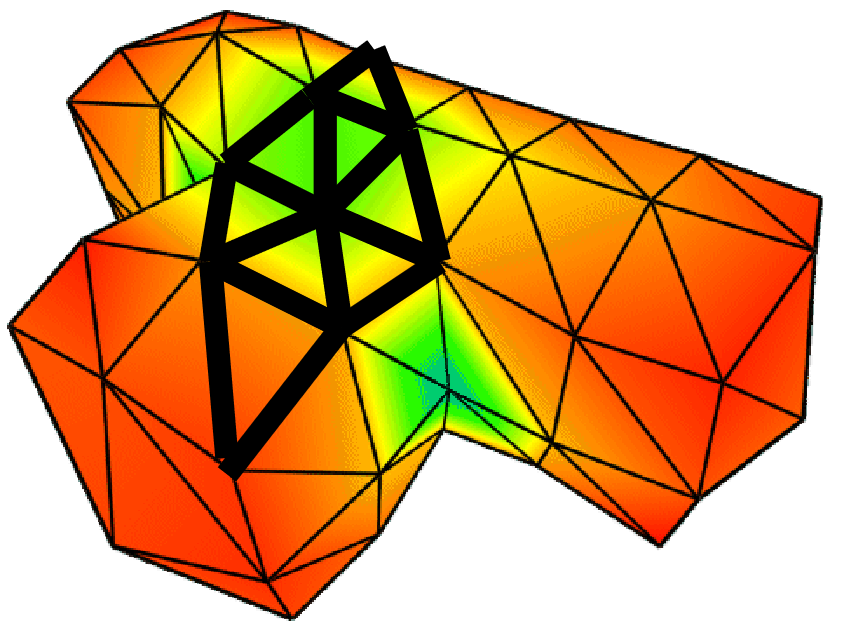
\includegraphics[width=0.3\columnwidth]{assets/arjun/butterfly.png}\\



